\documentclass[10pt]{article}
\usepackage[top=1.5in]{geometry}
% \usepackage[letterpaper, hmargin=0.75in, vmargin=0.75in]{geometry}
\usepackage{graphicx}
\usepackage{url}
\usepackage{hyperref}
\usepackage{listings}
\usepackage{pgf}
\usepackage{courier}
\usepackage{tabu}
\usepackage{booktabs}
\parindent 0in
\parskip 1.5ex
\usepackage{lastpage}
\usepackage{fancyhdr}
\usepackage{enumitem}
\usepackage{color}
\usepackage{amsmath}
\usepackage{mathpartir}
\usepackage{comment}
\usepackage{multicol}
\usepackage{pgf}
\usepackage{amsfonts}
\usepackage{tikz}
\usepackage{listings}
\usepackage{inconsolata}
\usepackage{pythonhighlight}
\usetikzlibrary{arrows,shapes,automata}
\lstset{ %
  numbers=none,numberstyle=\scriptsize,
  basicstyle=\ttfamily\small,commentstyle=\small\itshape,showstringspaces=false,breaklines=true}
\tikzstyle{block} = [rectangle, draw, fill=blue!20, 
    text width=5em, text centered, rounded corners, minimum height=2em]

\lstdefinelanguage{Dafny}{
  keywords={new, true, false, catch, function, return, null, var, if,
    in, while, else, reads, requires, decreases, ensures, then,
    returns, method, invariant, modifies, forall, exists, assume, assert,
    predicate, array, Length },
  %% keywordstyle=\color{blue}\bfseries,
  keywordstyle=\bfseries,
  ndkeywords={class, export, int, boolean, throw, implements, import, this, ::},
  ndkeywordstyle=\color{darkgray}\bfseries,
  identifierstyle=\color{black},
  sensitive=false,
  comment=[l]{//},
  morecomment=[s]{/*}{*/},
  %% commentstyle=\color{purple}\ttfamily,
  %% stringstyle=\color{red}\ttfamily,
  commentstyle=\ttfamily,
  stringstyle=\ttfamily,
  morestring=[b]',
  morestring=[b]"
}
\newcommand{\brac}[1]{\texttt{\textless #1\textgreater}}

\let\origthelstnumber\thelstnumber
\makeatletter
\newcommand*\Suppressnumber{%
  \lst@AddToHook{OnNewLine}{%
    \let\thelstnumber\relax%
     \advance\c@lstnumber-\@ne\relax%
    }%
}

\newcommand*\Reactivatenumber{%
  \lst@AddToHook{OnNewLine}{%
   \let\thelstnumber\origthelstnumber%
   \advance\c@lstnumber\@ne\relax}%
}
\makeatother

\newcommand{\atmostone}{\textit{at-most-one}}
\pagestyle{fancy}
\fancyhf{}
\renewcommand{\headrulewidth}{0pt}

\usepackage{tikz}
\newcommand*\circled[1]{\tikz[baseline=(char.base)]{
            \node[shape=circle,draw,inner sep=2pt] (char) {#1};}}

\newenvironment{solution}%
{
\noindent
{\bf Sample solution:}\\
}{}

\excludecomment{solution}

\begin{document}

\newgeometry{top=5.8in}
\copyright\ 2026 University of Waterloo\newline
\textbf{SE 465 --– Software Testing and Quality Assurance}\newline
\textbf{ECE 653 --– Software Testing, Quality Assurance \& Maintenance}\newline
Instructor: Patrick Lam \newline

\textbf{Instructions:}
\begin{itemize}[leftmargin=*]
	\setlength\itemsep{0em}
  \item You have \textbf{80 minutes} to complete the exam.
  \item You can refer to \textbf{printed or handwritten} material, e.g.,
    books, slides, notes, etc., as well as \textbf{reference} material saved on your computer.
  \item You may not do searches for information on the Internet (no browsers, please; local document viewers only).
  \item You may use Python and Python coverage tools.
  \item You may not ask anyone or any automated system (eg LLMs) for help with your exam, either in person or online.
  \item If information appears to be missing from a question, make a
    reasonable assumption, state your assumption, and proceed. 
\end{itemize}


\newpage
\restoregeometry

%\vspace*{8em}
\section*{Question 1: Short Answer (15 points)}

Answer these questions in one or two sentences. Each is worth 3 points.

\begin{enumerate}[label=(\alph*)]
\item [(a)] In general terms, why is static analysis subject to false positives but not dynamic analysis?\\[5em]
\item [(b)] In metamorphic testing, what do we do to validate an observed test output?\\[5em]
\item [(c)] When we compute a test suite's statement coverage, we often report a result as a percentage of
lines covered. Why is a percentage a more useful number than an absolute number of lines covered?\\[5em]
\item [(d)] Conversely, coverage-guided fuzzing does not need to know the number of statements that can
potentially be covered. Why not?\\[5em]
\item [(e)] With respect to extracting configuration grammars, what are 2 assumptions that the technique from the \emph{Fuzzing Book} rely on?
\end{enumerate}

\newpage
\begin{solution}
\begin{enumerate}[label=(\alph*)]
\item [(a)] I'm looking for something along the lines of: static analysis usually aims to
reason about all possible behaviours (thus including false positives),
while dynamic analysis only inspects what actually happens (so, no false positives)..
\item [(b)] We check that the observed output satisfies the required metamorphic relation. It is not mandatory
to use the term ``metamorphic relation'', but the answer should say something about the output being as expected
using what we know about the input.
\item [(c)] Can be compared across different source files.
\item [(d)] It is just aiming to increase the number of covered statements, and does not need to compare across files.
\item [(e)] Some answers: is a Python program, uses command line parameters, relies on \texttt{argparse}, uses it in a way that is similar to what the technique can read.
\end{enumerate}
\end{solution}

\newpage
%\vspace*{8em}
\section*{Question 2: Mutation Analysis (20 points)}
Consider the following function witten in the Python programming language.

\lstinputlisting[language=Python,numbers=left]{string\_conversion.py}

\begin{enumerate}[label=(\alph*)]
\item [(a)] (10 points) Propose inputs that achieve 100\% statement coverage of \texttt{add\_lists} as a series of calls to that function. Give the inputs in the same format as ``Examples'' above.

\item [(b)] (8 points) In class, we talked about how, in practice, tools generate mutants only for lines that have changed. Here, assume that line 18 was changed in the most recent commit. Propose two non-stillborn and non-equivalent mutants of line 18. Write down mutated versions of the code. Clearly indicate (with comments in the code) how you mutated the program and give a name for the mutation operator you applied (which you may make up).

\item [(c)] (10 points) Additionally, write unit tests that kill both of your mutants, in the same format as for part (a). Show that your tests succeed on the original program and fail
  on the mutant, e.g. by calculating and writing down outputs of the tests on the original and new code. You have a computer, so you are allowed to use Python to run code. If you added new test cases for this part, discuss whether they provide more insight than the ones for part (a). If you did not need to add new test cases, discuss what that says about statement coverage and mutation analysis on this example.

\end{enumerate}

\begin{solution}
We will accept answers that work for the truncated version as well as the full version. I apologize for the mix-up. I also meant for part (a) to be worth 2 points and not 10; the point change must have been due to some editing fiasco, but we will honour the posted point value and make Q2 out of 28 points.
  \begin{enumerate}[label=(\alph*)]
  \item This input yields 100\% statement coverage:
\begin{verbatim}
>>> print (string_conversion('a|@a^'))
['a', 'a', '']
\end{verbatim}
It's easy enough to verify this if you have a computer and measure the coverage on that input.
  \item original: \verb|token += literal_char|; \\
  potential mutant 1: \verb|token = literal_char| (modify assignment operator);\\
  potential mutant 2: \verb|token += c| (modify variable).

Other changes are possible as well.
  \item Using the provided test case kills my mutants, satisfying the question specification.

I've put outputs into a table:
  
%% {\scriptsize
%% \begin{tabular}{llll}
%% & original & mutant 1 & mutant 2 \\
%% provided input \verb+'@xone|uno^^|'+ & \verb+['one', 'unox', 'x', '', '']+ & \verb+['one', 'unox', 'x', '', '']+ & \verb+['one', 'uno^', '^', '', '']+ \\
%% input from (a) \verb+'a|@a^'+ & \verb+['a', 'a', '']+ & \verb+['a', 'a', '']+ & \verb+['a', '^', '']+
%% \end{tabular}
%% }

\begin{center}
\begin{tabular}{l|l|l}
& provided input \verb+'@xone|uno^^|'+ & input from (a)  \verb+'a|@a^'+ \\ \hline
original & \verb+['one', 'unox', 'x', '', '']+ & \verb+['a', 'a', '']+ \\
mutant 1 & \verb+['one', 'x, 'x', '', '']+ & \verb+['a', 'a', '']+ \\
mutant 2 & \verb+['one', 'uno^', '^', '', '']+ & \verb+['a', '^', '']+ \\
\end{tabular}
\end{center}

I didn't specify that you had to show that the mutants were non-stillborn, non-equivalent, and so you should not do that on this exam. But, since the mutants don't crash on at least one input (indeed, two), they are non-stillborn; and, we can show non-equivalence using the provided input for both of the mutants, since they return different output on the provided input.

As for the insight question, for the input I provided as my answer for part (a), that input provides less insight into the code than the provided test case, since it doesn't distinguish mutant 1 from the original. I'd conclude that 100\% statement coverage is not telling you much here.

Marking guide for TAs: Some marking infrastructure will help here. I found it easiest to create two copies of \verb+string_conversion+ and mutate the copies. Since we have to mark on both the truncated and intended versions, probably have six functions in all, and apply the mutations to different versions. The \texttt{\_\_main\_\_} should print the output from all of the functions. 

  \end{enumerate}
\end{solution}

%\newpage
%\vspace*{8em}
%(more question 2 answers)
\newpage
%\vspace*{8em}
\section*{Question 3: Random and Coverage-Guided Fuzzing (20 points)}

Here is a method. 
\begin{lstlisting}[language=Python,numbers=left]
def crash_midterm(inp:str) -> None:
    c = 0
    if len(inp) == 0:
        return
    if inp[0] >= '1' and inp[0] <= '9':
        c = int(inp[0])
    if c+4 <= len(inp) and inp[c] == '%':
        if inp[c+1] == '*':
            if inp[c+2] == '&':
                if inp[c+3] == '<':
                    raise Exception()
\end{lstlisting}

%% What is the common goal of evaluating test suites by their coverage, and coverage-guided fuzzing? Why do you need the denominator for evaluating test suites by coverage, but not for coverage-guided fuzzing?

\begin{enumerate}[label=(\alph*)]

\item [(a)] (2 points) What is an input that would cause this method to reach the \texttt{raise Exception()} statement? (Don't forget that you can check your answer on your computer!)
% "1%*^<"
\item [(b)] (4 points) Would you expect random fuzzing, as implemented in \texttt{fuzzer()} from L07 (with its default parameters, notably a \texttt{char\_start} of 32 and a \texttt{char\_range} of 32) to find the raised exception on \texttt{crash\_midterm()} in 100,000 trials? In at most two sentences, say why or why not.
% unlikely (but not impossible): the four comparisons require 1/32^4, which is 1 in 1 million, and there are other conditions too.
\item [(c)] (14 points) Work through enough calls to \texttt{MutationCoverageFuzzer.run()}, as described in Lecture 8, to reach the \texttt{Exception}. You must show at least 3 calls to \texttt{run()}. Start with the seed \texttt{[""]}. As you are working through the algorithm, you can choose any mutated input you want, but it has to be something that could be generated by the \texttt{MutationCoverageFuzzer} (explain how). Show the newly-generated input, along with the population and the coverage at each step. You can show the coverage as a set of line numbers from the above listing.
\end{enumerate}

\begin{solution}
\vspace*{-1em}
  \begin{enumerate}[label=(\alph*)]
\item [(a)] One can construct input \verb+"1%*&< "+.
\item [(b)] Unlikely but not impossible: each input has a 1/32 chance of matching, so we need $(1/32)^4$, which is about 1 million; you are running 100,000 trials. So, as a rough estimate, that's a 10\% chance. For this purpose, it's OK to ignore the gate at line 5, though you can include it in your calculation if you want.
\item [(c)]
\begin{verbatim}
(1) "" -- pop: [""], cov: {[1,2,3,4]}
(2) "aaaa" -- pop: ["", "aaaa"], cov: {[1,2,3,4], [1,2,3,5,7]}
(3) "1%*&<" -- pop: ["", "aaaa", "1%*&<"], cov: {[1,2,3,4], [1,2,3,5,7], [1,2,3,5,6,7,8,9,10,11]}
\end{verbatim}

(1) is the initial input.

The \texttt{MutationCoverageFuzzer} can then generate input \verb+"aaaa"+ through its parent \texttt{MutationFuzzer}'s \texttt{fuzz()} method calling \texttt{create\_candidate()}, drawing 4 trials (4 is between min 2 and max 10 mutations), each of which happens to call \verb+insert_random_character+ to insert an \texttt{a} into the candidate. (Feeling lucky?) This candidate adds coverage [2,3,5,7].

Since we know that we're trying to reach the input from (a), we can mutate input \verb+"aaaa"+ to reach that input through, for instance, 4 random deletions of the \verb+a+s and 5 random insertions of the characters in \verb+'1%*&< '+. Again, very lucky.
\end{enumerate}
\end{solution}

%\newpage
%\vspace*{8em}
%(more question 3 answers)
\newpage
\section*{Question 4: Oracles (15 points)}
Here is a Finite State Machine modelling a subway turnstile,
which controls access to the platforms. You have to insert a coin
to unlock the turnstile, at which point you can push the turnstile
to return to the initial locked position. The turnstile provides
methods \texttt{push()} and \texttt{coin()} for actions and function
\texttt{get\_state()} which returns either \texttt{LOCKED} or
\texttt{UNLOCKED}.
\begin{center}
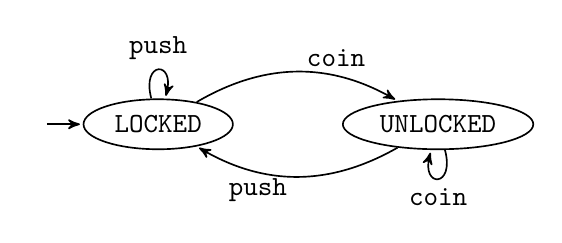
\begin{tikzpicture}[->,>=stealth',shorten >=1pt,auto,node distance=2.5cm,
                    semithick,initial text=]

  \node[initial,ellipse,draw]   (A)              {\texttt{LOCKED}};
  \node[ellipse,draw]           (B) [right of=A,xshift=3em] {\texttt{UNLOCKED}};
  
  \path (A) edge[bend left]              node[right,yshift=.5em] {\texttt{coin}} (B)
        (B) edge[bend left]              node[left,yshift=-.5em] {\texttt{push}} (A)
        (A) edge[loop above,min distance=5mm]              node {\texttt{push}} (A)
        (B) edge[loop below,min distance=5mm]              node {\texttt{coin}} (B);
\end{tikzpicture}
\end{center}

\begin{enumerate}[label=(\alph*)]
\item [(a)] (3 points) Give three specific examples of implicit oracles---observable
  behaviours of programs that always indicate that something is wrong with the program.
  An example should be no longer than a sentence.
  
\item [(b)] (4 points)
  Write test cases (4) that cover all of the state transitions for this FSM and check that the
  proper state is reached. Each test case may assume that it starts in the \texttt{LOCKED} state.

\item [(c)] (8 points) In the notes, it says that regression testing uses an earlier version as
  an oracle. Write a function, a change to that function, and a test case, such that the earlier
  version is a valid oracle to the new version; and, a change and test case such that the earlier
  version is not a valid oracle.
\end{enumerate}


\begin{solution}
\begin{enumerate}[label=(\alph*)]
\item [(a)] crash; uncaught exception; undefined behaviour as caught by a sanitizer; deadlock; assertion failure.
\item [(b)] Here are the test cases:

\begin{verbatim}
LOCKED --push--> LOCKED
Action: Call push()
Check: Assert get_state() == LOCKED

LOCKED --coin--> UNLOCKED
Action: Call coin()
Check: Assert get_state() == UNLOCKED

UNLOCKED --coin--> UNLOCKED
Action: Call coin() (to unlock), then call coin() again.
Check: Assert get_state() == UNLOCKED

UNLOCKED --push--> LOCKED
Action: Call coin() (to unlock), then call push().
Check: Assert get_state() == LOCKED
\end{verbatim}

\item [(c)] Original function:
\begin{python}
def calculate_total(price):
    return price + (price * 0.05)
\end{python}

New function where original function is a correct oracle:
\begin{python}
def calculate_total(price):
    tax_rate = 0.05
    return price * (1 + tax_rate)
\end{python}

New function where original function is not a correct oracle:
\begin{python}
def calculate_total(price):
    return price + (price * 0.10)
    \end{python}
Test case that works for both: \begin{verbatim} calculate_total(10) 
\end{verbatim}
\end{enumerate}
\end{solution}

\newpage
\section*{Question 5: Grammar Fuzzing (15 points)}

Here is the BNF grammar \texttt{PROCESS\_NUMBERS} from lecture,
\begin{python}
  { '<start>': ['<operator> <integers>'],
    '<operator>': ['--sum', '--min', '--max'],
    '<integers>': ['<integer>', '<integers> <integer>'],
    '<integer>': ['<digit-1>'],
    '<digit>': ['0', '1', '2', '3', '4', '5', '6', '7', '8', '9'],
    '<digit-1>': ['<digit>', '<digit><digit-1>'] }
\end{python}
and here is a modified subset of \texttt{EXPR\_GRAMMAR}.
\begin{python}
  { '<start>': ['<factor>'],
    '<factor>': ['+<factor>', '-<factor>', '<integer>.<integer>.<integer>'],
    '<integer>': ['8'] }
\end{python}

\begin{enumerate}[label=(\alph*)]
\item [(a)] (5 points) You are allowed to run Python code on this midterm, so you can see that \texttt{symbol\_cost} of
\brac{integers} is 4. Write down an explanation of why this is the case.
\item [(b)] (8 points) Write down the steps that \texttt{expand\_node\_by\_cost} takes, when
  \texttt{choose} is \texttt{max}
  and \texttt{choose\_node\_expansion()} is random. Your \texttt{DerivationTree} is \{ ('\brac{factor}', None) \}.
\item [(c)] (2 points) Give an example of a grammar where \brac{start} has symbol cost \texttt{inf}.
% no, let's do a thing where we do the max-cost expansion instead of the current (c).
%% \item [(c)] (3 points) Give an example of a grammar where the minimum length path from \brac{start}
%%   to a terminal is 3. What is the shortest string that can be generated from this grammar?
\end{enumerate}

\begin{solution}
\begin{enumerate}[label=(\alph*)]
\item [(a)] The cost is determined by:
\texttt{integers} $\rightarrow$ \texttt{integer} $\rightarrow$ \texttt{digit-1} $\rightarrow$ \texttt{digit} $\rightarrow$ \texttt{terminal}
\item [(b)] First, it fetches the expansions from the grammar, and computes their costs as well as the subtrees that would ensue from choosing each expansion.

\verb!'+<factor>'! and \verb!'-<factor>'! have equal cost, and this cost is greater than the cost of \verb!'<integer><integer><integer>'!. Since choose is max, it draws randomly from \verb!'+<factor>'! or \verb!'-<factor>'!, and expands \verb+<factor>+ with the subtree with the chosen signed \verb+factor+.

If the computer draws \verb!'+<factor>'!, we get \verb!('<factor>', [('+', []), ('<factor>', None)])!.

If the computer draws \verb!'-<factor>'!, we get \verb!('<factor>', [('-', []), ('<factor>', None)])!.
\item [(c)]
\begin{verbatim}
<’start’>: [‘<start>’]
\end{verbatim}
\end{enumerate}

\end{solution}
%\newpage
%\vspace*{8em}
%(more question 5 answers)

\newpage
\section*{Question 6: Delta Debugging (20 points)}

This is delta debugger output for the \texttt{MysteryRunner} in Lecture 11 on a randomly generated input, rounded up to make the numbers nicer. Call the original input, in test \#1, ``\texttt{inp}''.
\begin{verbatim}
Test #1 ' 7:,>((/$$-/->.;.=;(.%!:50#7*8=$&&=$9!%6(4=&69\':\'<3+0-3.24#7=!&60)2/+";+<7+1<2!4$>92
              +$1<(3%&5\'\'>#000' 100 FAIL
Test #2 '3+0-3.24#7=!&60)2/+";+<7+1<2!4$>92+$1<(3%&5\'\'>#000' 50 PASS
Test #3 " 7:,>((/$$-/->.;.=;(.%!:50#7*8=$&&=$9!%6(4=&69':'<" 50 PASS
Test #4 '0#7*8=$&&=$9!%6(4=&69\':\'<3+0-3.24#7=!&60)2/+";+<7+1<2!4$>92+$1<(3%&5\'\'>#000' 75 FAIL
Test #5 "0#7*8=$&&=$9!%6(4=&69':'<1<2!4$>92+$1<(3%&5''>#000" 50 PASS
Test #6 '0#7*8=$&&=$9!%6(4=&69\':\'<3+0-3.24#7=!&60)2/+";+<7+' 50 FAIL
Test #7 '3+0-3.24#7=!&60)2/+";+<7+' 25 PASS
Test #8 "0#7*8=$&&=$9!%6(4=&69':'<" 25 PASS
Test #9 '!%6(4=&69\':\'<3+0-3.24#7=!&60)2/+";+<7+' 38 FAIL
\end{verbatim}
You probably want to talk about the current value of \texttt{n} as computed in the \texttt{DeltaDebuggingReducer}.

\begin{enumerate}[label=(\alph*)]
\item [(a)] (2 point) Explain how you can get the substrings for test \#2 and test \#3, as a function of \texttt{inp}.
% remove half
\item [(b)] (4 points) What about test \#4? What is it derived from?
% double n, now remove a quarter of test 1
\item [(c)] (8 points) What is the relationship between test \#4 and tests \#5/\#6? Why are there only 2 tests of length 50 after test \#4, rather than 3 tests?
% tests #5 and #6 each remove one-third of test #4, but there is a cached result which means that the third test doesn't run
\item [(d)] (6 points) How is the input for test \#9 computed, as a function of previous tests?
% back up to #6, remove 1/4 of that string
\end{enumerate}

\begin{solution}
\begin{enumerate}[label=(\alph*)]
\item [(a)] \verb+test3 = inp1[0:50]; test2(inp) = inp1[50:100]+
\item [(b)] \verb!test4 = inp1[25:50] + inp1[50:75] + inp1[75:100]!
\item [(c)] \verb!test5 = inp4[0:25] + inp4[50:75]!; \verb!test6 = inp4[0:25] + inp4[25:50]!; the missing test was not executed because the cache had already seen it and gave the answer.
\item [(d)] \verb!test9 = inp6[13:25] + inp6[25:38] + inp6[38:50]!
\end{enumerate}
\end{solution}


\end{document}


%%% Local Variables:
%%% mode: latex
%%% TeX-master: t
%%% End:
